% Options for packages loaded elsewhere
\PassOptionsToPackage{unicode}{hyperref}
\PassOptionsToPackage{hyphens}{url}
%
\documentclass[
]{book}
\usepackage{amsmath,amssymb}
\usepackage{lmodern}
\usepackage{iftex}
\ifPDFTeX
  \usepackage[T1]{fontenc}
  \usepackage[utf8]{inputenc}
  \usepackage{textcomp} % provide euro and other symbols
\else % if luatex or xetex
  \usepackage{unicode-math}
  \defaultfontfeatures{Scale=MatchLowercase}
  \defaultfontfeatures[\rmfamily]{Ligatures=TeX,Scale=1}
\fi
% Use upquote if available, for straight quotes in verbatim environments
\IfFileExists{upquote.sty}{\usepackage{upquote}}{}
\IfFileExists{microtype.sty}{% use microtype if available
  \usepackage[]{microtype}
  \UseMicrotypeSet[protrusion]{basicmath} % disable protrusion for tt fonts
}{}
\makeatletter
\@ifundefined{KOMAClassName}{% if non-KOMA class
  \IfFileExists{parskip.sty}{%
    \usepackage{parskip}
  }{% else
    \setlength{\parindent}{0pt}
    \setlength{\parskip}{6pt plus 2pt minus 1pt}}
}{% if KOMA class
  \KOMAoptions{parskip=half}}
\makeatother
\usepackage{xcolor}
\IfFileExists{xurl.sty}{\usepackage{xurl}}{} % add URL line breaks if available
\IfFileExists{bookmark.sty}{\usepackage{bookmark}}{\usepackage{hyperref}}
\hypersetup{
  pdftitle={Reproducible guide},
  pdfauthor={Anthony Davidson},
  hidelinks,
  pdfcreator={LaTeX via pandoc}}
\urlstyle{same} % disable monospaced font for URLs
\usepackage{longtable,booktabs,array}
\usepackage{calc} % for calculating minipage widths
% Correct order of tables after \paragraph or \subparagraph
\usepackage{etoolbox}
\makeatletter
\patchcmd\longtable{\par}{\if@noskipsec\mbox{}\fi\par}{}{}
\makeatother
% Allow footnotes in longtable head/foot
\IfFileExists{footnotehyper.sty}{\usepackage{footnotehyper}}{\usepackage{footnote}}
\makesavenoteenv{longtable}
\usepackage{graphicx}
\makeatletter
\def\maxwidth{\ifdim\Gin@nat@width>\linewidth\linewidth\else\Gin@nat@width\fi}
\def\maxheight{\ifdim\Gin@nat@height>\textheight\textheight\else\Gin@nat@height\fi}
\makeatother
% Scale images if necessary, so that they will not overflow the page
% margins by default, and it is still possible to overwrite the defaults
% using explicit options in \includegraphics[width, height, ...]{}
\setkeys{Gin}{width=\maxwidth,height=\maxheight,keepaspectratio}
% Set default figure placement to htbp
\makeatletter
\def\fps@figure{htbp}
\makeatother
\setlength{\emergencystretch}{3em} % prevent overfull lines
\providecommand{\tightlist}{%
  \setlength{\itemsep}{0pt}\setlength{\parskip}{0pt}}
\setcounter{secnumdepth}{5}
\usepackage{booktabs}
\ifLuaTeX
  \usepackage{selnolig}  % disable illegal ligatures
\fi
\usepackage[]{natbib}
\bibliographystyle{plainnat}

\title{Reproducible guide}
\usepackage{etoolbox}
\makeatletter
\providecommand{\subtitle}[1]{% add subtitle to \maketitle
  \apptocmd{\@title}{\par {\large #1 \par}}{}{}
}
\makeatother
\subtitle{Draft}
\author{Anthony Davidson}
\date{2022-02-14}

\usepackage{amsthm}
\newtheorem{theorem}{Theorem}[chapter]
\newtheorem{lemma}{Lemma}[chapter]
\newtheorem{corollary}{Corollary}[chapter]
\newtheorem{proposition}{Proposition}[chapter]
\newtheorem{conjecture}{Conjecture}[chapter]
\theoremstyle{definition}
\newtheorem{definition}{Definition}[chapter]
\theoremstyle{definition}
\newtheorem{example}{Example}[chapter]
\theoremstyle{definition}
\newtheorem{exercise}{Exercise}[chapter]
\theoremstyle{definition}
\newtheorem{hypothesis}{Hypothesis}[chapter]
\theoremstyle{remark}
\newtheorem*{remark}{Remark}
\newtheorem*{solution}{Solution}
\begin{document}
\maketitle

{
\setcounter{tocdepth}{1}
\tableofcontents
}
\hypertarget{nice-label}{%
\chapter{Overview}\label{nice-label}}

This guide is really a combination of reproducible resources for graduate research and beyond using RMarkdown through RStudio.

Welcome!

This is a minimal example of a book based on R Markdown and \textbf{bookdown} (\url{https://github.com/rstudio/bookdown}).

This template provides a skeleton file structure that you can edit to create your book.

The contents inside the .Rmd files provide some pointers to help you get started, but feel free to also delete the content in each file and start fresh.

Additional resources:

The \textbf{bookdown} book: \url{https://bookdown.org/yihui/bookdown/}

The \textbf{bookdown} package reference site: \url{https://pkgs.rstudio.com/bookdown}

If you prefer text as the link instead of a numbered reference use: \protect\hyperlink{nice-label}{any text you want can go here}.

\hypertarget{working-with-this-resource}{%
\section{Working with this resource}\label{working-with-this-resource}}

\hypertarget{description}{%
\section{Description}\label{description}}

Using tools like git for version control and knitr for dynamic figure generation are great steps forward towards better research transparency and reproducibility.

But there are also steps to be made in improving code and preparing data for re-use. These steps don't necessarily involve the use of new tools, but instead would be the result of applying ``best practice'' guidelines.

We aim to begin compiling resources here. This is only a start, and we'd encourage anyone to suggest further guidelines, particularly those that are specific to various statistical software packages.

\begin{center}\rule{0.5\linewidth}{0.5pt}\end{center}

\hypertarget{guidelines-for-writing-code}{%
\section{Guidelines for writing code}\label{guidelines-for-writing-code}}

\textbf{Very useful manual}:

\href{http://web.stanford.edu/~gentzkow/research/CodeAndData.pdf}{Gentzkow and Shapiro, ``Code and Data for the Social Sciences: A Practitioner's Guide'' (including section ``RA Manual: Notes on Writing Code.'') 2014}

We'd recommend reading the full guide, but briefly outline the sections of ``RA Manual: Notes on Writing Code'' here so as to give a preview. We also include one example from each section, but there are many other examples in the original paper.

\begin{center}\rule{0.5\linewidth}{0.5pt}\end{center}

\hypertarget{code-should-be-logical}{%
\subparagraph{Code should be logical}\label{code-should-be-logical}}

\begin{itemize}
\tightlist
\item
  Despise redundancy
\item
  Separate functional code and metadata
\item
  Use the right data structures
\item
  Make your functions shy
\item
  Use overriding methods instead of switches where appropriate
\end{itemize}

\emph{Example: use the right data structures}

Instead of writing a function like:

\begin{verbatim}
myfunction <- function(name, surname, age, height) {
  if (age < 18) {}
}
\end{verbatim}

We can use a structure like an object or array for that.

\begin{verbatim}
myfunction <- function(person) {
  if (person.age < 18) { }
}
\end{verbatim}

This would make the code easier to read and maintain.

\begin{center}\rule{0.5\linewidth}{0.5pt}\end{center}

\hypertarget{code-should-be-readable}{%
\subparagraph{Code should be readable}\label{code-should-be-readable}}

\begin{itemize}
\tightlist
\item
  Keep it short
\item
  Order your functions for linear reading
\item
  Choose descriptive names
\item
  Use white space and indents to make code scannable
\item
  Pay special attention to coding algebra
\item
  Make logical switches intuitive
\item
  Use enough comments and no more
\item
  Be consistent
\item
  Avoid commands that make code hard to read
\end{itemize}

\emph{Example: choose descriptive names}

It might be easier for other users to read and adapt existing code if the variables, folders, classes and other elements have simple and intuitive names. So prefer writing code like:

\begin{verbatim}
calculate_status <- function(person) {}
\end{verbatim}

Rather than:

\begin{verbatim}
cs <- function(p) {}
\end{verbatim}

\begin{center}\rule{0.5\linewidth}{0.5pt}\end{center}

\hypertarget{code-should-be-robust}{%
\subparagraph{Code should be robust}\label{code-should-be-robust}}

\begin{itemize}
\tightlist
\item
  Check for errors
\item
  Write tests
\end{itemize}

\emph{Example: check for errors}

Users can use your code with different parameters and in different environments. It is a good practice to include code that check for erroneous values and provide clear feedback.

\begin{verbatim}
myfunction <- function(x, y) {
  return x / y;
}

myfunction <- function(x, y) {
  if (y == 0) 
    return 'y must be different than zero!';
  return x / y; 
}
\end{verbatim}

Of course you can also write tests to make sure your verifications are working correctly ;-)

\begin{center}\rule{0.5\linewidth}{0.5pt}\end{center}

\hypertarget{code-should-be-efficient}{%
\subparagraph{Code should be efficient}\label{code-should-be-efficient}}

\begin{itemize}
\tightlist
\item
  Profile slow code relentlessly
\item
  Store ``too much'' output from slow code
\item
  Separate slow code from fast code
\end{itemize}

\begin{center}\rule{0.5\linewidth}{0.5pt}\end{center}

\hypertarget{packages-and-libraries-needed}{%
\section{Packages and libraries needed:}\label{packages-and-libraries-needed}}

\hypertarget{introduction}{%
\chapter{Introduction}\label{introduction}}

Modern challenges of reproducibility in research, particularly computational reproducibility {[}cite{]}, have produced a lot of discussion in papers, blogs and videos, some of which are listed \href{https://github.com/davan690/reproducible-guidebook/blob/main/sections/references/index.md}{here}.

\hypertarget{bes-guidelines}{%
\section{BES guidelines}\label{bes-guidelines}}

In 2017 The britich ECological Society produced a set of reproduciblity guidelines \href{https://github.com/BES2016Workshop/guidebook}{here}.

{[}pdf and notes coming\ldots.{]}

\hypertarget{whats-a-reproducible-report}{%
\section{What's a reproducible report?}\label{whats-a-reproducible-report}}

For the purposes of this guide, a report is a scientific document that contains not only the text that makes up the manuscript, but also the code that generates the figures and the statistics that are reported in your manuscript. Ideally, the report is part of a self-contained project that may contain your data, your initial exploratory analyses, the final product, and the code needed to generate them.

This manuscript can be a scientific article, a conference presentation, a technical report, or a document to share your progress with your collaborators. The end product may not show any code and therefore it may not look like it was generated differently from other documents.

Typically a report contains code for data manipulation, data analysis, and figure generation alongside the text that constitutes the heart of the report. Because of this hybrid nature, if left unchecked, this mix can lead to a big mess that can be difficult to maintain and debug. In this guide, we will provide you with some advice on how to keep your report manageable.

Box xx: What is the difference between repeatability and reproducibility?

\textbf{Repeatability} describes how close are the results of an experiment conducted under the same conditions (same instruments, same operators, etc.). \textbf{Reproducibility} describes how close are the results of an experiment conducted under similar but different conditions. Repeatability ensures that you would obtain similar results when running your code on your own laptop at different times; while reproducibility ensures that giving your code to someone else would allow them to obtain the same results as yours.

\hypertarget{why-a-reproducible-report}{%
\section{Why a reproducible report?}\label{why-a-reproducible-report}}

Did you ever have to redo an analysis 6 months later, and it was difficult. You forgot which one of the 15 files with ``final'' in their names was really the one you should have used? Have you ever spent several hours assembling an intricate figure with your favorite drawing program, just to realize that your collaborators had forgotten to send you the latest batch of data? Writing a reproducible report alleviates some of these hurdles. By automating how the figures and the statistics in your report are generated, you are leaving a code trail that you, your collaborators, or your readers can take, and that leads to your original data. This path to the raw data increases the transparency of your science. However, in order for the six-month-in-the-future you, your collaborators, and your readers, to be able to take this path, it is important that you organize your code and your data files consistently.

Not only does writing a reproducible report increase the transparency of your science, it reduces the mistakes that result from copying and pasting across software. Keeping the content of your manuscript in sync with the output of your statistical program is challenging. By specifying directly the output of your model in your text, it is easier to make sure you are referring to the correct model with the correct parameters. To be the devil's advocate, one could argue that the additional code that will need to be written to integrate the results within the text could lead to additional errors. However, these bugs are possible to detect (contrary to mistakes done by copying and pasting the correct numbers), and their consequences can be assessed by re-running the code generating the manuscript after fixing them.

Writing a reproducible report allows you to tell a much richer story than the narrative in the report by itself does. The text in your report does not usually show the different approaches and analyses you have tried before coming up with the final results. With a reproducible report, you can provide readers who want to know more about how you obtained the results in your paper, the approaches you tried and the their results. These can be included as supplementary material or tagged in the history of your version control system.

To make your report reproducible, your code will need to be self-contained. As a consequence, you will be able to re-use the code you wrote for one project in another one. Therefore, if initially it might slow you down to make your code reproducible, it is an investment in the future as you will be able to re-use and build upon it in the future. Additionally, others might be able to also re-use your code, and apply it for their own data. Your efforts may speed up the overall scientific process (you or your colleagues won't need to re-invent the wheel for each project), and you could get more citations on your papers.

It can feel daunting to get started with writing a reproducible report because of the technical skills and knowledge required. However, a partially reproducible report is better than a non-reproducible one. So each step you take towards reproducibility is worth taking, and sets you up to take the next one for the next project.

\hypertarget{how-to-deal-with-citations}{%
\subsection{How to deal with citations?}\label{how-to-deal-with-citations}}

You need two things: a BibTeX file that contains all the citations you use in your manuscript and a CSL (Citation Style Language) file that specifies the format of your citation. Software citation managers such as Zotero or Mendeley provide options to generate BibTeX files for your citations. CSL files exist for most journals, and can be downloaded from: \url{https://www.zotero.org/styles}. This is a convenient search interface provided by Zotero but you do not need to use Zotero to download or use these files.

\hypertarget{where-can-i-find-more-information}{%
\section{Where can I find more information?}\label{where-can-i-find-more-information}}

\begin{itemize}
\tightlist
\item
  The RStudio Markdown website: \url{http://rmarkdown.rstudio.com/}
\item
  The bookdown website: \url{https://bookdown.org/yihui/bookdown/}
\end{itemize}

\hypertarget{documenting-and-managing-dependencies}{%
\chapter{Documenting and managing dependencies}\label{documenting-and-managing-dependencies}}

Reproducibility is also about making sure someone else can re-use your code to obtain the same results as yours. Understanding why your analysis may not lead to the same results on a different computer can be useful to determine how careful you need to be in documenting your setup.

For someone else to be able to reproduce the results included in your report, you need to provide more than the code and the data. You also need to document the exact versions of all the packages, libraries, and software you used, and potentially your operating system as well as your hardware.

R itself is very stable, and the core team of developer takes backward compatibility (that old code works with recent version of R) very seriously. However, default values in some functions have changed, and new functions get introduced regularly. If you wrote your code on a recent version of R and give it to someone who hasn't upgraded recently, they may not be able to run your code. If R itself is stable, the packages are generally much less stable. New functionalities get introduced with each versions, some functions get deprecated, and defaults options change. Code written for one version of a package may produce very different results with a more recent version.

Documenting and managing the dependencies of your project correctly can be a complicated. However, even simple documentation that helps others understand the setup you used can have a big impact. Here we present three levels of complexity to document the dependencies for your projects.

\hypertarget{show-the-packages-you-used}{%
\section{Show the packages you used}\label{show-the-packages-you-used}}

With R, the simplest (but useful and important) approach to document your dependencies is to report the output of \texttt{sessionInfo()} (or \texttt{devtools::session\_info()}). Among other information, this will show all the packages (and their versions) that are loaded in the session you used to run your analysis. If someone wants to recreate your analysis, they will know which packages they will need to install.

\hypertarget{use-packages-that-help-recreate-your-setup}{%
\section{Use packages that help recreate your setup}\label{use-packages-that-help-recreate-your-setup}}

The \texttt{checkpoint} package provides a way to download all the packages at a given date from CRAN. Thus, from the output provided by \texttt{sessionInfo()}, they could recreate your setup. It however makes two important assumptions: all your packages were up-to-date with CRAN at the time of your analysis; you were not using packages that are not available from CRAN (e.g.~the development version of a package directly from a git repository).

Another approach is to use the \texttt{packrat} package. This package creates a library (a collection of packages) directly within your analysis directory. It increases the size of your project as all the source code for the packages is included, but it ensures that someone can recreate more reliably the same environment as the one you used for your analysis. It also makes it easier because the installation of these packages is fully automated for the person wanting to have the same setup.

\hypertarget{use-containers-to-share-your-setup}{%
\section{Use containers to share your setup}\label{use-containers-to-share-your-setup}}

A step further in complexity is to use Docker. With Docker you recreate an entire operating system with all the software, data, and packages needed for your analysis. It is more technical to set up but it allows you to distribute the exact same environment as the one you used. If you want others to be able reproduce your results, and your analysis depends on software that can be difficult to install, it is an option that might be worth exploring.

Original content from ``Althea ArchMiller''

\hypertarget{methods}{%
\chapter{Methods}\label{methods}}

You can add parts to organize one or more book chapters together. Parts can be inserted at the top of an .Rmd file, before the first-level chapter heading in that same file.

Add a numbered part: \texttt{\#\ (PART)\ Act\ one\ \{-\}} (followed by \texttt{\#\ A\ chapter})

Add an unnumbered part: \texttt{\#\ (PART\textbackslash{}*)\ Act\ one\ \{-\}} (followed by \texttt{\#\ A\ chapter})

Add an appendix as a special kind of un-numbered part: \texttt{\#\ (APPENDIX)\ Other\ stuff\ \{-\}} (followed by \texttt{\#\ A\ chapter}). Chapters in an appendix are prepended with letters instead of numbers.

\hypertarget{footnotes-and-citations}{%
\chapter{Footnotes and citations}\label{footnotes-and-citations}}

\hypertarget{footnotes}{%
\section{Footnotes}\label{footnotes}}

Footnotes are put inside the square brackets after a caret \texttt{\^{}{[}{]}}. Like this one \footnote{This is a footnote.}.

\hypertarget{citations}{%
\section{Citations}\label{citations}}

Reference items in your bibliography file(s) using \texttt{@key}.

For example, we are using the \textbf{bookdown} package \citep{R-bookdown} (check out the last code chunk in index.Rmd to see how this citation key was added) in this sample book, which was built on top of R Markdown and \textbf{knitr} \citep{xie2015} (this citation was added manually in an external file book.bib).
Note that the \texttt{.bib} files need to be listed in the index.Rmd with the YAML \texttt{bibliography} key.

The RStudio Visual Markdown Editor can also make it easier to insert citations: \url{https://rstudio.github.io/visual-markdown-editing/\#/citations}

\hypertarget{blocks}{%
\chapter{Blocks}\label{blocks}}

\hypertarget{equations}{%
\section{Equations}\label{equations}}

Here is an equation.

\begin{equation} 
  f\left(k\right) = \binom{n}{k} p^k\left(1-p\right)^{n-k}
  \label{eq:binom}
\end{equation}

You may refer to using \texttt{\textbackslash{}@ref(eq:binom)}, like see Equation \eqref{eq:binom}.

\hypertarget{theorems-and-proofs}{%
\section{Theorems and proofs}\label{theorems-and-proofs}}

Labeled theorems can be referenced in text using \texttt{\textbackslash{}@ref(thm:tri)}, for example, check out this smart theorem \ref{thm:tri}.

\begin{theorem}
\protect\hypertarget{thm:tri}{}\label{thm:tri}For a right triangle, if \(c\) denotes the \emph{length} of the hypotenuse
and \(a\) and \(b\) denote the lengths of the \textbf{other} two sides, we have
\[a^2 + b^2 = c^2\]
\end{theorem}

Read more here \url{https://bookdown.org/yihui/bookdown/markdown-extensions-by-bookdown.html}.

\hypertarget{callout-blocks}{%
\section{Callout blocks}\label{callout-blocks}}

The R Markdown Cookbook provides more help on how to use custom blocks to design your own callouts: \url{https://bookdown.org/yihui/rmarkdown-cookbook/custom-blocks.html}

\hypertarget{github-and-git}{%
\section{github and git}\label{github-and-git}}

Reproducibility practices for scientific code are sorely needed. Now is the time to come together as a scientific community to decide what works and what doesn't.

One of the best ways to collaborate on a digital project is to use the version control system, git, and have it freely available through an online hosting system, in this case \href{https://github.com/}{github}. Every file that is used to build this guide is on a \href{https://github.com/ropensci/reproducibility-guide}{repository called reproducibility-guide on github}.

There are several ways to contribute to this website. You don't have to contribute code. No matter if you are a programmer new to science, or a scientist new to programming, your perspective is needed for the advancement of scientific reproducibility.

\hypertarget{issues}{%
\section{Issues}\label{issues}}

One way to begin contributing is to start an \href{https://github.com/ropensci/reproducibility-guide/issues?state=open}{issue}. Issues are how we discuss the project. It can be as large as changing the entire structure of the site, or small, like adding a new tool to the Tools section.

Everyone who watches the project is alerted when an issue has been established, and everyone can comment on it. If you have an idea for making the site better, or just want to start a discussion on reproducibility in sciences, please start a new issue.

If you're not sure where to start, take a look at \href{https://github.com/ropensci/reproducibility-guide/issues?state=open}{already started issues}. Feel free to voice your opinion on any issue already mentioned, come join the discussion!

If you understand the basics of git, maybe you would like to take action and fix the issue by adding code to the repository.

\hypertarget{contributing-to-codebase}{%
\section{Contributing to Codebase}\label{contributing-to-codebase}}

Each collaborative project on github has an ecosystem, so the rules for collaborating are different depending on the project. Often housed in a CONTRIBUTING.md file, there are rules that have been adapted to suit the functionality of the project. For our project, we are flexible on how you contribute and encourage newbie git collaborators: everyone has to start somewhere. Here is a general guide for how you can contribute to the basecode for this site. If you are a beginning git user, this may seem a bit confusing, but we promise it becomes clear after trying it.

\hypertarget{tiny-tutorial-on-contributing-to-repositories}{%
\subsection{Tiny Tutorial on Contributing to Repositories}\label{tiny-tutorial-on-contributing-to-repositories}}

\emph{(requires base knowledge of git. Remixed from Karl Broman's \href{http://kbroman.github.io/github_tutorial/pages/fork.html}{github Guide - Contribute to Someone's repository}}

\begin{itemize}
\item
  Say you want to contribute changes to our code repository.
\item
  Go to the repository on github. (This site is from \texttt{ropensci}, and is called \texttt{reproducibility-guide}, you'll find it at \texttt{https://github.com/ropensci/reproducibility-guide}.
\item
  Click the fork button at the top right.
\item
  You'll now have your own copy of that repository in your github account.
\item
  Open a terminal/shell.
\item
  Type

\begin{verbatim}
 $ git clone https://github.com/username/reproducibility-guide.git
\end{verbatim}
\end{itemize}

where \texttt{username} is \emph{your} username.

\begin{itemize}
\item
  You'll now have a local copy of \emph{your version} of that repository called ``origin''
\item
  Add a connection to the original owner's repository and calling it ``master''.

\begin{verbatim}
  $ git remote add master https://github.com/ropensci/reproducibility-guide.git
\end{verbatim}
\item
  You can check if this worked with the command. You should see the connection to \emph{your version} of the repository and the ropensci ``master''
  version.

\begin{verbatim}
  $ git remote -v
\end{verbatim}
\item
  Now you can make changes to files. The main branch for the Reproducibility Guide site is \texttt{gh-pages}. You may also start another branch for to work on. To check which branch you are on type \texttt{git\ branch}.
\item
  \texttt{git\ add} and \texttt{git\ commit} those changes
\item
  \texttt{git\ push} them back to \href{http://github.com}{github}. These will go
  to \emph{your version} of the repository.
\item
  Go to \emph{your version} of the repository on github.
\item
  Click the green ``Pull Request'' button at the top of the page.
\item
  Note that the ropensci repository will be on the left and \emph{your repository} will be on the right.
\item
  Give a short explanation of the changes and click the ``Send pull request'' button.
\end{itemize}

\hypertarget{pulling-others-changes}{%
\section{Pulling others' changes}\label{pulling-others-changes}}

\begin{itemize}
\item
  Before you make further changes to the repository, you should check that your version is up to date relative to your friend's version.
\item
  Go into the directory for the project and type:

\begin{verbatim}
  $ git pull ropensci master
\end{verbatim}
\end{itemize}

This will pull down and merge all of the changes that your friend has made.

\begin{itemize}
\item
  Now push them back to your github repository.

\begin{verbatim}
  $ git push
\end{verbatim}
\end{itemize}

\hypertarget{add-yourself-to-the-contributors-section}{%
\section{Add yourself to the contributors section}\label{add-yourself-to-the-contributors-section}}

Now that you have contributed, you can add yourself to the \href{http://ropensci.github.io/reproducibility-guide/contributors/}{list of contributors}. The file to add your name to is located in the contributors folder in the main directory, just add your name to the index.md file housed \href{https://github.com/ropensci/reproducibility-guide/tree/gh-pages/contributors}{here}.

\hypertarget{resources}{%
\section{Resources}\label{resources}}

\href{http://kbroman.github.io/github_tutorial/}{Full git/github} - Karl Broman

\href{http://code.tutsplus.com/tutorials/how-to-collaborate-on-github--net-34267}{How to Collaborate on github} - tuts+

\hypertarget{captioned-figures-and-tables}{%
\section{Captioned figures and tables}\label{captioned-figures-and-tables}}

Figures and tables \emph{with captions} can also be cross-referenced from elsewhere in your book using \texttt{\textbackslash{}@ref(fig:chunk-label)} and \texttt{\textbackslash{}@ref(tab:chunk-label)}, respectively.

See Figure \ref{fig:nice-fig}.

\begin{figure}

{\centering 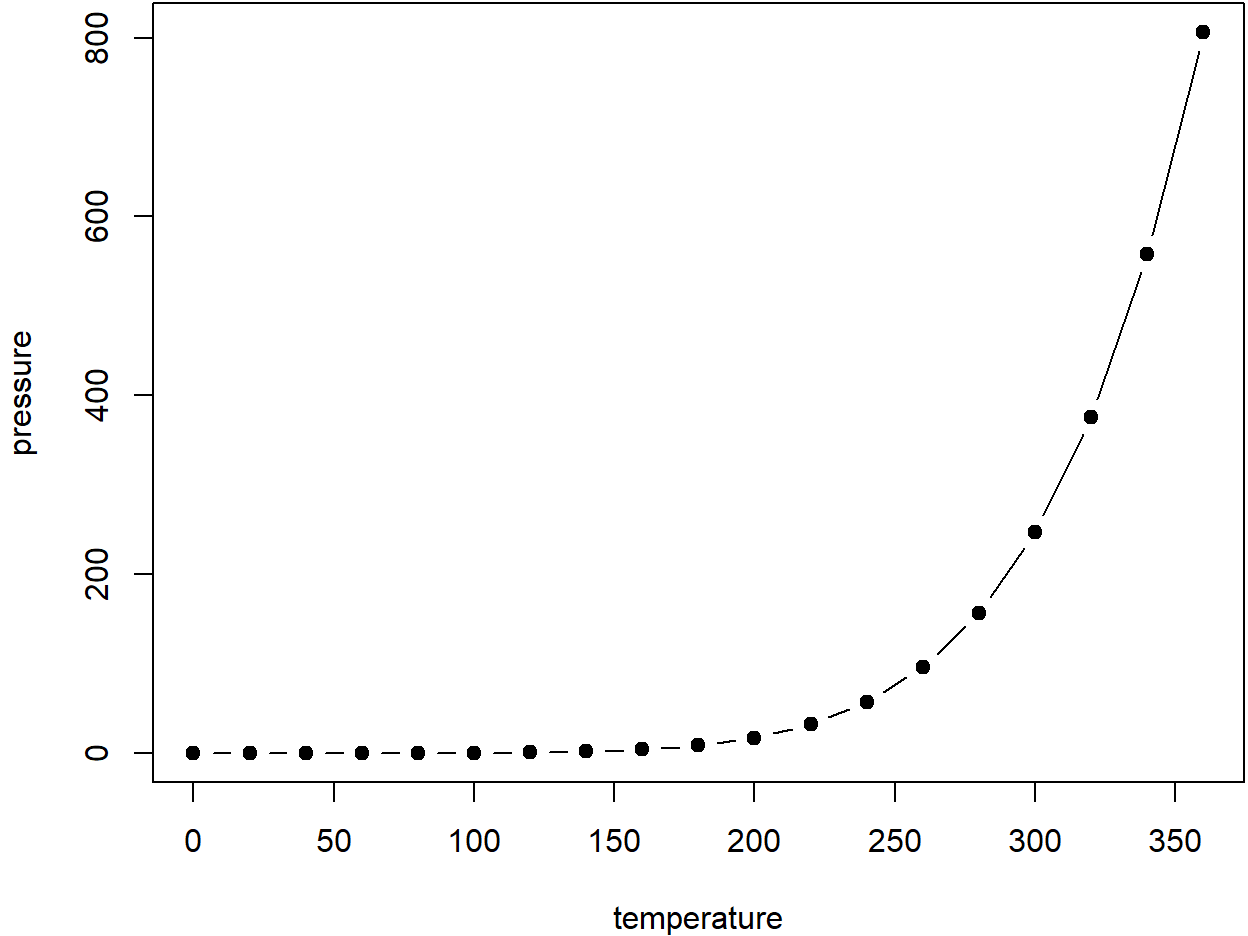
\includegraphics[width=0.8\linewidth]{figures/nice-fig-1} 

}

\caption{Here is a nice figure!}\label{fig:nice-fig}
\end{figure}

Don't miss Table \ref{tab:nice-tab}.

\begin{table}

\caption{\label{tab:nice-tab}Here is a nice table!}
\centering
\begin{tabular}[t]{rr}
\toprule
temperature & pressure\\
\midrule
0 & 0.0002\\
20 & 0.0012\\
40 & 0.0060\\
60 & 0.0300\\
80 & 0.0900\\
\addlinespace
100 & 0.2700\\
120 & 0.7500\\
140 & 1.8500\\
160 & 4.2000\\
180 & 8.8000\\
\bottomrule
\end{tabular}
\end{table}

\hypertarget{how-to-do-a-report-using-rmarkdown}{%
\section{How to do a report using RMarkdown?}\label{how-to-do-a-report-using-rmarkdown}}

Programming languages typically used by scientistics for data analysis have libraries or packages that can be used to generate reproducible reports. The most popular ones are Jupyter Notebooks for scientists who primarily use python and RMarkdown for those who use R. While they both share many commonalities, their implementation and everyday applications differ. Here, we focus on RMarkdown.

RMarkdown is a file format (typically saved with the \texttt{.Rmd} extension) that can contain: a YAML header (see next section), text, code chunks, and inline code. The \texttt{.rmarkdown} package converts this file into a report most commonly into HTML or PDF.

The \texttt{.rmarkdown} package automates a multi-step process (Fig. xx). Under the hood, it calls the \texttt{.knitr} package that converts the Rmd file into a markdown file. In the process, \texttt{.knitr} takes all the code chunks and the inline code, run them through R (or other programs), capture their output, and incorporates them in the report. Afterwards, \texttt{.rmarkdown} calls the pandoc program (it is an external program that is not related to R) that can take the markdown file and converts to a variety of formats. For pandoc to generate PDF files, you will need a functional \href{https://www.latex-project.org/get/}{installation of LaTeX} that you will need to install separately.

The \texttt{bookdown} package comes in to take care of numbering the figures and tables, as well as dealing with citations. As its name suggests, this package can be used to author books, but it is also well-suited to help generating reports.

\hypertarget{the-yaml-header}{%
\subsection{the YAML header}\label{the-yaml-header}}

The YAML header is at the top of your file, it is delineated by three dashes (\texttt{-\/-\/-}) at the top and at the bottom of it. It is optional, but can be used to specify:

\begin{itemize}
\tightlist
\item
  the characteristics of your document: the title, authors, date of creation.
\item
  the arguments to pass to pandoc to control the format of the output as
  well as additional information such as the bibliography file and the
  formatting of the list of references.
\item
  parameters for your report: for instance, you can specify a parameter such that your report will only use a subset of your data so the final product will be generated quickly when you are developing the code for your project. Once your code is working, you can switch to the full dataset.
\end{itemize}

\hypertarget{code-chunks}{%
\subsection{Code chunks}\label{code-chunks}}

Code chunks are interspersed within the text of the report. They are delineated by three backticks (\texttt{\$\textasciigrave{}\textasciigrave{}\textasciigrave{}\$}) at the top and at the bottom of it. The top backticks are followed by a curly bracket that specify: (1) the language in which the code chunk is written, (2) the name of the chunk (optional but good practice), (3) \texttt{knitr} options that control whether and how the code, the output, or the figure are interpreted and displayed. Everything that comes after the name of the chunk has to be a valid R expression: the strings need be quoted, the arguments are separated by commas, and logical values (\texttt{TRUE}/\texttt{FALSE}) need to be capitalized.

\hypertarget{how-to-deal-with-figures}{%
\subsection{How to deal with figures?}\label{how-to-deal-with-figures}}

The \texttt{knitr} package provides many options to finely control how your figures are going to be generated. Some of \texttt{knitr}'s options can be set individually for each chunk or be set globally. For a reproducible report, it is common practice to have chunk at the beginning of the report that sets default options for the figures. It is also usually a good place to load all the packages you will need for your analysis. For instance the following chunk will do the following:

\begin{itemize}
\tightlist
\item
  all the figures generated by the report will be placed in the \texttt{figures/} sub-directory
\item
  all the figures will be 6.5 x 4 inches and centered in the text.
\end{itemize}

Additionally, this chunk will be named \texttt{figuresetup}, and we use the \texttt{echo=FALSE} option so the code for the chunk will not be displayed in the report, and use the \texttt{include=FALSE} option so no output produced by this chunk will be included in the report.

For our figures, we can now do

\begin{figure}

{\centering 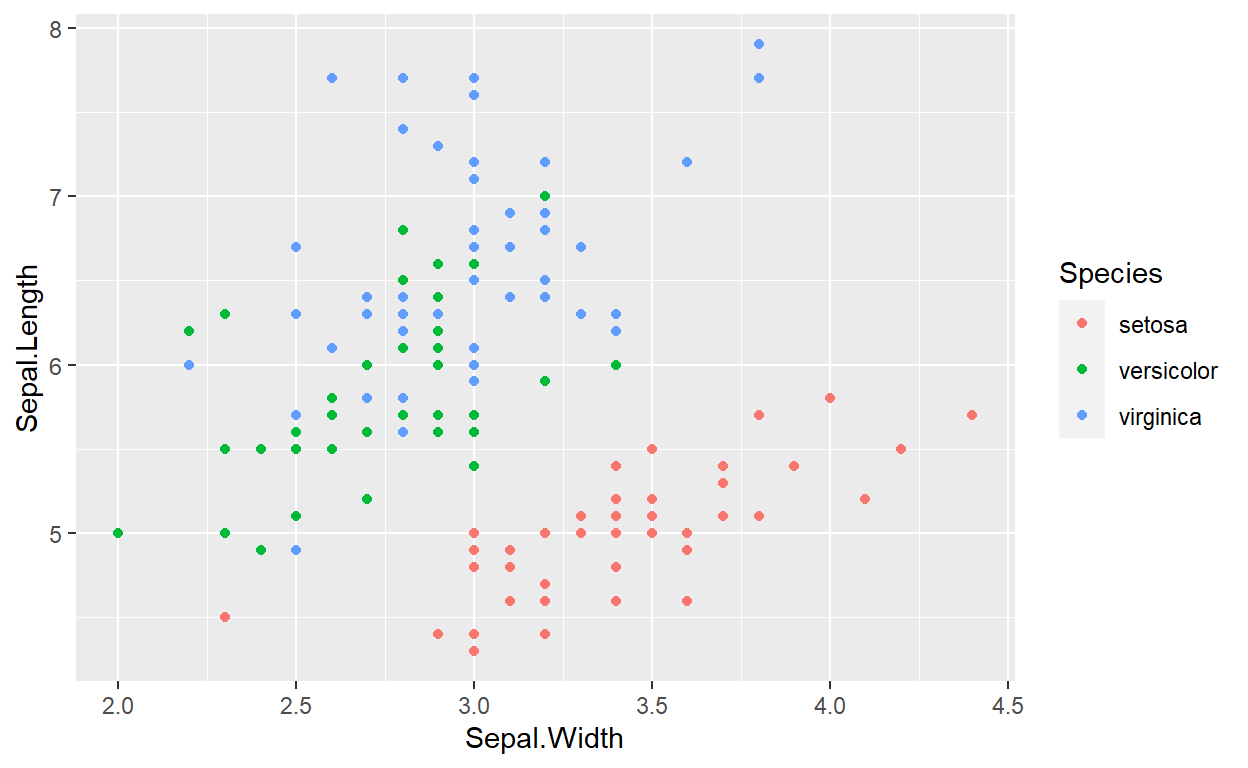
\includegraphics{figures/sepalwidthlength-1} 

}

\caption{Relation between sepal width and length in three species of Iris.}\label{fig:sepalwidthlength}
\end{figure}

When this file will be processed, it will create an image file (\texttt{figures/sepalwidthlength.png}) with the default dimension and the caption specified by the value of the \texttt{fig.cap} argument. You can use markdown formatting within the captions of your figures. This figure will have the label \texttt{fig:sepalwidthlength} that we will be able to use for cross referencing (see below).

If you wish to incorporate a figure that is not generated by code (a photo of your field site or study organism), using the function \texttt{\#knitr::include\_graphics()} takes care of many details for you, and generates labels and captions as if it was generated by code.

\begin{center}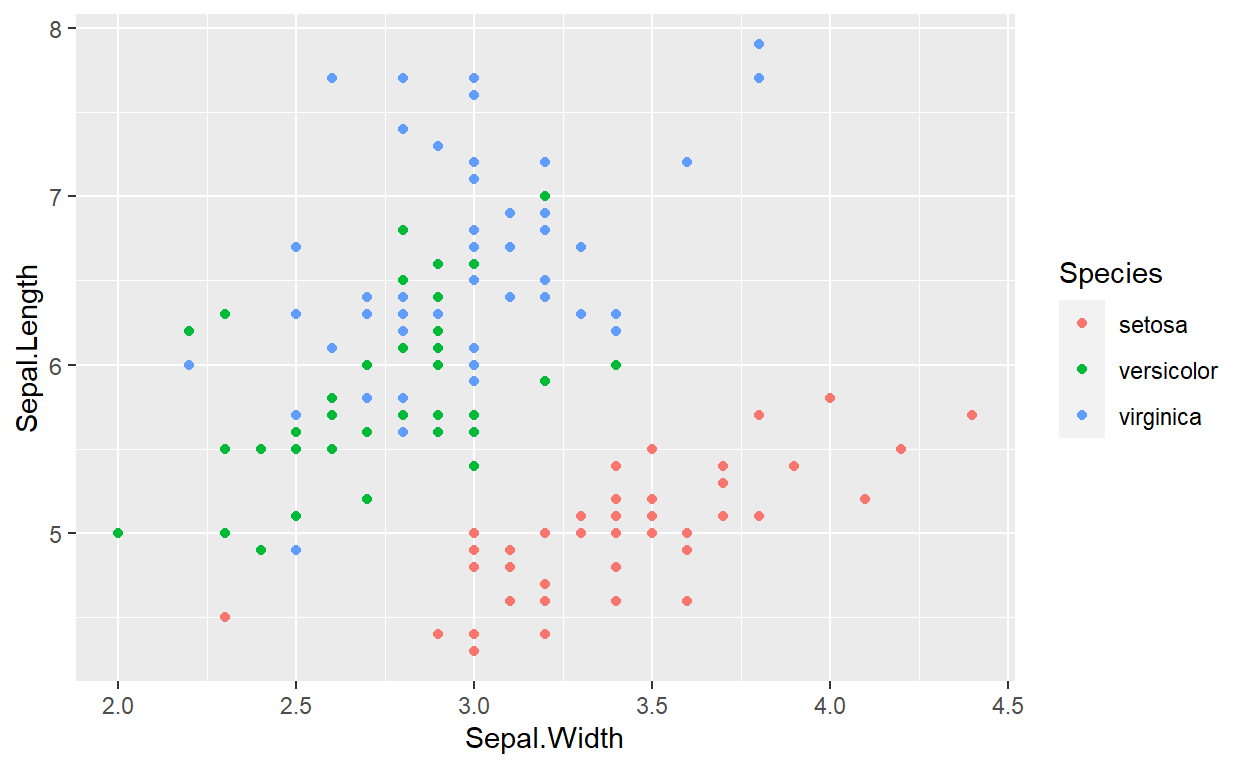
\includegraphics[width=17.33in]{figures/iris} \end{center}

\hypertarget{how-to-deal-with-tables}{%
\subsection{How to deal with tables?}\label{how-to-deal-with-tables}}

To generate tables, \texttt{knitr} comes with the function \texttt{kable} that might be sufficient to make simple tables to represent data frames within your report. However, there are many packages that provide more sophisticated approaches to display and format tabular data within your reports. This \href{https://hughjonesd.github.io/huxtable/design-principles.html}{page} provides an overview of the capabilities of the different packages.

\hypertarget{sharing-your-book}{%
\chapter{Sharing your book}\label{sharing-your-book}}

Additional resources for reference

\hypertarget{publishing}{%
\section{Publishing}\label{publishing}}

HTML books can be published online, see: \url{https://bookdown.org/yihui/bookdown/publishing.html}

\hypertarget{pages}{%
\section{404 pages}\label{pages}}

By default, users will be directed to a 404 page if they try to access a webpage that cannot be found. If you'd like to customize your 404 page instead of using the default, you may add either a \texttt{\_404.Rmd} or \texttt{\_404.md} file to your project root and use code and/or Markdown syntax.

\hypertarget{metadata-for-sharing}{%
\section{Metadata for sharing}\label{metadata-for-sharing}}

Bookdown HTML books will provide HTML metadata for social sharing on platforms like Twitter, Facebook, and LinkedIn, using information you provide in the \texttt{index.Rmd} YAML. To setup, set the \texttt{url} for your book and the path to your \texttt{cover-image} file. Your book's \texttt{title} and \texttt{description} are also used.

This \texttt{gitbook} uses the same social sharing data across all chapters in your book- all links shared will look the same.

Specify your book's source repository on GitHub using the \texttt{edit} key under the configuration options in the \texttt{\_output.yml} file, which allows users to suggest an edit by linking to a chapter's source file.

Read more about the features of this output format here:

\url{https://pkgs.rstudio.com/bookdown/reference/gitbook.html}

Or use:

Welcome!

This is a minimal example of a book based on R Markdown and \textbf{bookdown} (\url{https://github.com/rstudio/bookdown}).

This template provides a skeleton file structure that you can edit to create your book.

The contents inside the .Rmd files provide some pointers to help you get started, but feel free to also delete the content in each file and start fresh.

Additional resources:

The \textbf{bookdown} book: \url{https://bookdown.org/yihui/bookdown/}

The \textbf{bookdown} package reference site: \url{https://pkgs.rstudio.com/bookdown}

There are many many different resources on reproducible workflows. This document collects the current resources avaliable with a strong focus on \href{https://cran.r-project.org/}{R} and ( \href{https://rmarkdown.rstudio.com/}{RMarkdown}; \href{https://www.r-bloggers.com/composing-reproducible-manuscripts-using-r-markdown/}{blog here}).

I have started \href{}{this repository} from a combination of different git repositories:

\begin{itemize}
\tightlist
\item
  \href{https://github.com/BES2016Workshop/guidebook}{BES guidelines}
\end{itemize}

My workflow has a distinctly ecological feel along with the tidyverse approach of \href{https://style.tidyverse.org/index.html}{tooling}. I apologise for this in advance.
If you are not a \href{https://cran.r-project.org/}{R} user I would recommend modifying this workflow or finding another workflow with the same components but in your field.

\hypertarget{r-resources}{%
\chapter{R resources}\label{r-resources}}

Since the development of \href{https://cran.r-project.org/}{R} and \href{https://rstudio.com/}{RStudio} (and a magnitude of other IT changes happening at the same time) there are now tools for working with issues to do with \href{https://www.nature.com/news/1-500-scientists-lift-the-lid-on-reproducibility-1.19970}{reproducibility}. There are many blogs from a simple web search.
Here is a collection of the posts I have drawn inspiration from:

\begin{itemize}
\item
  \href{https://www.r-bloggers.com/}{R bloggers posts}: This is a collection of the current blogs on \href{https://www.r-bloggers.com}{R bloggers}.
\item
  \href{https://maraaverick.rbind.io/2017/09/r-workflow-fun/}{R workflow}: Mara Averick has a post that looks better than this and has many of the same resources just published a few years ago.
\item
  \href{https://methodsblog.com/2016/10/05/reproducibility-with-r/}{Methods in Ecology}: A good blog that goes with the reproducible guidebook (2018).
\item
  \href{https://csgillespie.github.io/efficientR/workflow.html}{workflow general tips}

  \begin{itemize}
  \tightlist
  \item
    \textbf{Key points}
  \end{itemize}

  \begin{enumerate}
  \def\labelenumi{\arabic{enumi}.}
  \tightlist
  \item
    Start without writing code but with a clear mind and perhaps a pen and paper. This will ensure you keep your objectives at the forefront of your mind, without getting lost in the technology.
  \item
    Make a plan. The size and nature will depend on the project but time-lines, resources and `chunking' the work will make you more effective when you start.
  \item
    Select the packages you will use for implementing the plan early. Minutes spent researching and selecting from the available options could save hours in the future.
  \item
    Document your work at every stage: work can only be effective if it's communicated clearly and code can only be efficiently understood if it's commented.
  \item
    Make your entire workflow as reproducible as possible. knitr can help with this in the phase of documentation. \href{https://csgillespie.github.io/efficientR/workflow.html}{Reference here}
  \end{enumerate}
\item
  \href{https://community.rstudio.com/t/data-science-project-template-for-r/3230}{Data Science and R/Python}
\item
  \href{https://timogrossenbacher.ch/2017/07/a-truly-reproducible-r-workflow/}{Truely reproducible}
\item
  \href{https://uoftcoders.github.io/rcourse/lec16-rmarkdown.html}{EEB313H1}
\item
  \href{https://swcarpentry.github.io/good-enough-practices-in-scientific-computing/}{Good enough practices for Scientific Computing}
\item
  \href{https://www.r-bloggers.com/reproducible-research-when-your-results-cant-be-reproduced/}{Pitfalls to non-reproducible research}: This is a nice simple post on the three danger zones: R session context; OS context; Data versioning.
\item
  \href{https://www.r-bloggers.com/what-is-reproducible-research/}{What is it?}: From Rbloggers.
\item
  \href{https://www.r-bloggers.com/stencila-an-office-suite-for-reproducible-research/}{Truely reproducible web}
\item
  \href{https://peerj.com/collections/50-practicaldatascistats/}{PeerJ stats help}
\item
  \href{http://blog.jom.link/implementation_basic_reproductible_workflow.html}{Implmentation guide}: Great post. I have used much of this for my workflow.
\item
  \href{https://www.one-tab.com/page/HngnpHOKRpuiqeQEB7_B7A}{A list of sites I haven't sorted yet}
\end{itemize}

\hypertarget{databases-for-reproducible-packages}{%
\subsubsection{Databases for reproducible packages}\label{databases-for-reproducible-packages}}

\begin{itemize}
\item
  \href{https://ropensci.org/about/}{rOpenSci} is a non-profit initiative founded in 2011 by Karthik Ram, Scott Chamberlain, and Carl Boettiger to make scientific data retrieval reproducible. Over the past seven years we have developed an ecosystem of open source tools, we run annual conferences, and review community developed software.
\item
  \href{https://cran.r-project.org/web/views/ReproducibleResearch.html}{The Reproducible Research CRAN Task View}
\end{itemize}

Both of these pages are doing a great job at producing searchable interface for reproducible packages in R with documentation.

\hypertarget{journals}{%
\chapter{Journals}\label{journals}}

\hypertarget{plos}{%
\paragraph{PLOS}\label{plos}}

\begin{itemize}
\item
  \href{http://journals.plos.org/plosbiology/article?id=10.1371/journal.pbio.1001745}{Best practices for Scientific Computing}
\item
  \href{http://journals.plos.org/ploscompbiol/article?id=10.1371/journal.pcbi.1003285}{10 simple rules for reproducible computational research}
\item
  \href{http://journals.plos.org/ploscompbiol/article?id=10.1371/journal.pcbi.1000424}{A quick guide to organizing computational biology projects}
\item
  \href{http://journals.plos.org/ploscompbiol/article?id=10.1371/journal.pcbi.1005097}{Ten Simple Rules for Digital Data Storage}
\end{itemize}

\hypertarget{coding-groups}{%
\section{Coding groups}\label{coding-groups}}

\begin{itemize}
\item
  \href{https://github.com/UofTCoders}{Uni of Toronto Coders}
  -\href{https://github.com/UofTCoders/rcourse}{R course}
\item
  \href{http://stat545.com/Classroom/}{UBC statistics course}
\end{itemize}

With all the resources above I have created a evolving ``workflow'' for my research.

\begin{itemize}
\tightlist
\item
  \href{https://cyberhelp.sesync.org/basic-git-lesson/2016/08/25/}{Distributed Workflows}: This is a class on reproducible workflows in RStudio. Ian Carroll says:
\end{itemize}

\emph{A single collaboration model -- the centralized workflow -- dominates collaborative research. There is a central hub, and everyone synchronizes their work to it. A number of researchers are nodes -- consumers of that hub -- and synchronize to that one place.}

{[}1{]} \textbf{Scholarly Context Not Found: One in Five Articles Suffers from Reference Rot}, Klein et al, \url{https://doi.org/10.1371/journal.pone.0115253}

{[}2{]} \textbf{Software citation principles}, Smith et al, \url{https://doi.org/10.7717/peerj-cs.86}

{[}3{]} \textbf{Code publication and citation}, Croucher et al, \url{https://doi.org/10.5281/zenodo.801586}

\hypertarget{resources-1}{%
\chapter{Resources}\label{resources-1}}

Over the past few years there has been a hige development of reproducible research tools using R.

\hypertarget{rstudio-tools-and-packages}{%
\section{RStudio tools and packages}\label{rstudio-tools-and-packages}}

Since the development of R and RStudio (and a magnitude of other IT changes happening at the same time) there are now tools for working with issues to do with \href{https://www.nature.com/news/1-500-scientists-lift-the-lid-on-reproducibility-1.19970}{reproducibility}. There are many blogs from a simple web search.

Here is a collection of the posts I have drawn inspiration from:

\begin{itemize}
\tightlist
\item
  \href{https://www.r-bloggers.com/reproducible-research-and-r-workflow/}{R bloggers post}: Jeromy Anglim
\item
  \href{https://cyberhelp.sesync.org/basic-git-lesson/2016/08/25/}{Reproducible workflows in RStudio}
\item
  \href{https://maraaverick.rbind.io/2017/09/r-workflow-fun/}{R workflow}: Mara Averick
\item
  \href{https://methodsblog.com/2016/10/05/reproducibility-with-r/}{Methods in Ecology}
\item
  \href{https://csgillespie.github.io/efficientR/workflow.html}{workflow general tips}
\item
  \href{https://community.rstudio.com/t/data-science-project-template-for-r/3230}{Data Science and R/Python}
\item
  \href{https://timogrossenbacher.ch/2017/07/a-truly-reproducible-r-workflow/}{Truely reproducible}
\item
  \href{https://uoftcoders.github.io/rcourse/lec16-rmarkdown.html}{EEB313H1}
\end{itemize}

\hypertarget{scientific-publications}{%
\section{Scientific publications}\label{scientific-publications}}

There are many many different posts on reproducible workflows. This document collects the current resources available in R and RMarkdown. I have developed this document from a combination of different git repositories:

\begin{itemize}
\item
  BES guidelines as a start
\item
  Added Wickhams etc paper
\item
  Best practices for Scientific Computing (\url{http://journals.plos.org/plosbiology/article?id=10.1371/journal.pbio.1001745})
\item
  Good enough practices for Scientific Computing (\url{https://swcarpentry.github.io/good-enough-practices-in-scientific-computing/})
\item
  10 simple rules for reproducible computational research: \url{http://journals.plos.org/ploscompbiol/article?id=10.1371/journal.pcbi.1003285}
\item
  A quick guide to organizing computational biology projects: \url{http://journals.plos.org/ploscompbiol/article?id=10.1371/journal.pcbi.1000424}
\item
  Ten Simple Rules for Digital Data Storage (\url{http://journals.plos.org/ploscompbiol/article?id=10.1371/journal.pcbi.1005097})
\item
  The Reproducible Research CRAN Task View: (\url{https://cran.r-project.org/web/views/ReproducibleResearch.html})
\end{itemize}

\hypertarget{workflow-options}{%
\section{Workflow options}\label{workflow-options}}

However because of this my workflow has a distinctly ecological feel along with the tidyverse approach of \href{https://style.tidyverse.org/index.html}{tooling}. I apologise for this in advance. If you are not a R user I would recommend finding another workflow with the same components.

\begin{itemize}
\item
  \href{https://peerj.com/preprints/3192/}{Packaging data publication}
\item
  \href{}{Tidytools package}
\end{itemize}

\hypertarget{files-within-this-repository}{%
\chapter{Files within this repository}\label{files-within-this-repository}}

Resources include the templates and resources within this repository.

\begin{verbatim}
 [1] "checklist"          "collaborationGuide" "copyrightLicensing"
 [4] "dataSharing"        "dataStorage"        "introduction"      
 [7] "metaData"           "references"         "tools"             
[10] "versionControl"     "workflows"          "writingCode"       
\end{verbatim}

\hypertarget{checklist}{%
\section{Checklist}\label{checklist}}

Reproduciblity can occur at every step in the history of your project. How easy will it be for others or your future self to answer these questions?

\hypertarget{documentation}{%
\subsection{Documentation}\label{documentation}}

❏ Is it clear where to begin? (e.g., can someone picking a project up see where to start running it)\\
❏ can you determine which file(s) was/were used as input in a process that produced a derived file?\\
❏ Who do I cite? (code, data, etc.)

❏ Is there documentation about every result?

❏ Have you noted the exact version of every external application used in the process?

❏ For analyses that include randomness, have you noted the underlying random seed(s)?

❏ Have you specified the license under which you're distributing your content, data, and code?

❏ Have you noted the license(s) for others peoples' content, data, and code used in your analysis?

\hypertarget{organization}{%
\subsection{Organization}\label{organization}}

❏ Which is the most recent data file/code?

❏ Which folders can I safely delete?

❏ Do you keep older files/code or delete them?

❏ Can you find a file for a particular replicate of your research project?

❏ Have you stored the raw data behind each plot?

❏ Is your analysis output done hierarchically? (allowing others to find more detailed output underneath a summary)

❏ Do you run backups on all files associated with your analysis?\\
❏ How many times has a particular file been generated in the past?\\
❏ Why was the same file generated multiple times?\\
❏ Where did a file that I didn't generate come from?

\hypertarget{automation}{%
\subsection{Automation}\label{automation}}

❏ Are there lots of manual data manipulation steps are there?

❏ Are all custom scripts under version control?

❏ Is your writing (content) under version control?

\hypertarget{publication}{%
\subsection{Publication}\label{publication}}

❏ Have you archived the exact version of every external application used in your process(es)?

❏ Did you include a reproducibility statement or declaration at the end of your paper(s)?

❏ Are textual statements connected/linked to the supporting results or data?

❏ Did you archived preprints of resulting papers in a public repository?

❏ Did you release the underlying code at the time of publishing a paper?

❏ Are you providing public access to your scripts, runs, and results?

\hypertarget{references}{%
\subsubsection{References}\label{references}}

\emph{Originally created at the \href{https://github.com/Reproducible-Science-Curriculum/Reproducible-Science-Hackathon-Dec-08-2014}{Reproducibility Hackathon} 2014}

This takes a combination of reproducible guides, inputs them into a bookdown project and begins to write R scripts to access the dynamic database of reproducibility literature underneath it.

\hypertarget{coding-groups-1}{%
\section{Coding groups}\label{coding-groups-1}}

\begin{itemize}
\tightlist
\item
  \href{https://github.com/UofTCoders}{Uni of Toronto Coders}
  -\href{https://github.com/UofTCoders/rcourse}{R course}
\end{itemize}

\hypertarget{software-options}{%
\chapter{Software options}\label{software-options}}

rOpenSci \href{https://ropensci.org/about/}{is a non-profit initiative founded in 2011 by Karthik Ram, Scott Chamberlain, and Carl Boettiger to make scientific data retrieval reproducible. Over the past seven years we have developed an ecosystem of open source tools, we run annual unconferences, and review community developed software.}

They have produced a great interface for reproducible packages in R with documentation. The key software and packages I use for my workflow are:

\hypertarget{file-building}{%
\section{File building}\label{file-building}}

Im not sure what this is actually meant to represent but I see these options as packages making \href{https://wlandau.github.io/2016/06/14/workflow/}{packages}

\hypertarget{packrat}{%
\subsection{packrat}\label{packrat}}

In mid-August of 2016, Eric Nantz of the R-Podcast converted me to packrat (by Kevin Ushey and others at RStudio), a package that lengthens the shelf life of R projects. \href{https://rstudio.github.io/packrat/}{Packrat} maintains local snapshots of dependencies so that your project won't break when external packages are updated. Just be sure your current working directory is the root directory of your project when you run remake::make() or the Makefile. Also, if you use a shell.sh with your Makefile, be sure to modify module load R so that it points to the version of R corresponding to your packrat library. You can learn more about packrat with the hands-on walkthrough.

\hypertarget{projecttemplate}{%
\subsection{ProjectTemplate}\label{projecttemplate}}

\begin{itemize}
\tightlist
\item
  \href{https://cran.r-project.org/web/packages/ProjectTemplate/ProjectTemplate.pdf}{ProjectTemplate} and the webpage is \href{http://projecttemplate.net/}{here}.
\item
  A workshop using this \href{https://github.com/jeromyanglim/leuven2016rworkshop}{package}
\end{itemize}

\hypertarget{packages}{%
\section{Packages}\label{packages}}

Hadley wickham book on \href{http://r-pkgs.had.co.nz/}{R Packages}.

\hypertarget{r}{%
\subsection{R}\label{r}}

\begin{itemize}
\tightlist
\item
  \href{https://github.com/benmarwick/rrtools}{rrtools}
\end{itemize}

\hypertarget{version-control}{%
\section{Version control}\label{version-control}}

\hypertarget{markdown}{%
\section{Markdown}\label{markdown}}

  \bibliography{book.bib,packages.bib,references.bib,reproduce.bib}

\end{document}
